\documentclass[12pt, a4paper]{article}
\usepackage[german]{babel}
\usepackage{import}
\usepackage{blindtext}
\usepackage{titling}
\usepackage{datetime}
\usepackage[dvipsnames]{xcolor}
\usepackage{amsmath, pgfplots}
\usepackage[hidelinks, breaklinks]{hyperref}
% Links auf Gleitumgebungen springen nicht zur Beschriftung,
% sondern zum Anfang der Gleitumgebung
\usepackage[figure]{hypcap}
\usepackage{fancyhdr}
\usepackage{float}
% limit floats to stay in their section
\usepackage[section]{placeins}
\usepackage[top=2.5cm, bottom=2.5cm, left=2.5cm, right=2.5cm]{geometry}
% \usepackage{showframe}
\usepackage{xcolor}

% add subsubsub-section
\usepackage{titlesec}
\setcounter{secnumdepth}{3}

\usepackage{subcaption}
\usepackage{graphicx}
\graphicspath{{./rsc/img/(1)}{./rsc/img/(2)}}

% Umlaut-Unterstützung
% siehe auch https://www.namsu.de/Extra/befehle/Umlaute.html
% !! inputenc VOR biblatex laden
\usepackage[utf8]{inputenc} % Umlaut-Unterstützung
\usepackage[T1]{fontenc} % Umlaut-Unterstützung für Silbentrennung

\usepackage[style=verbose-ibid,backend=bibtex]{biblatex}
\addbibresource{\jobname.bib}

% Enable use of \abs{value} and \norm{value} in formulas
% See https://tex.stackexchange.com/a/43009
\usepackage{mathtools}

\DeclarePairedDelimiter\abs{\lvert}{\rvert}
\DeclarePairedDelimiter\norm{\lVert}{\rVert}

% Swap the definition of \abs* and \norm*, so that \abs
% and \norm resizes the size of the brackets, and the 
% starred version does not.
\makeatletter
\let\oldabs\abs
\def\abs{\@ifstar{\oldabs}{\oldabs*}}

\let\oldnorm\norm
\def\norm{\@ifstar{\oldnorm}{\oldnorm*}}
\makeatother

% Use \cdot instead of '*' by default
\usepackage{etoolbox}

\makeatletter
\patchcmd{\@fnsymbol}{*}{\ast}{}{}
\patchcmd{\@fnsymbol}{*}{\ast}{}{}
\patchcmd{\@fnsymbol}{*}{\ast}{}{}
\makeatother

\mathcode`\*=\cdot

\pgfplotsset{compat=1.18}
% optimize pgfplots compilation: export plot, then import into document to
% prevent unnecessary recompilation
\usepgfplotslibrary{groupplots, external}
\tikzexternalize[prefix=cache/]
% import additional pgfplots/tikz libraries (for plotting)
\usepgfplotslibrary{polar, patchplots, colorbrewer}
\usetikzlibrary{calc, positioning}

% import after tikz configuration
\usepackage[textwidth=3.7cm,german]{todonotes}
\setlength{\marginparwidth}{3.7cm}
% prevent tikz externalization of todo notes since this does not work together
\makeatletter
\renewcommand{\todo}[2][]{\tikzexternaldisable\@todo[#1]{#2}\tikzexternalenable}
\makeatother
\newcommand\draftred[1]{\textcolor{red}{#1}}


% Debug-Anzeige von übervollen Boxen:
%! FIXME: remove for shipping
% \overfullrule=1 mm
% \tikzifexternalizing{\setkeys{Gm}{showframe=false}}{}

\setlength{\headheight}{15pt}
\addtolength{\topmargin}{-10pt}

\title{\textbf{Geschwindigkeitsmessung von Fahrzeugen durch Audio-Analyse}}
\author{Levin Fober}
\date{\today}

\pagestyle{fancy}

\renewcommand{\sectionmark}[1]{\markright{\thesection~- ~#1}}

\fancyhf{} % reset everything
\fancyhead[L]{\rightmark} % rightmark = current section; leftmark = current chapter
\fancyfoot[C]{\thepage}
% \fancyfoot[C]{\theauthor}
\fancyfoot[L]{}

\AtEndDocument{
    \FloatBarrier
    \newpage

    \thispagestyle{plain}

    \hfill
    \vfill

    \noindent
    \rule{\textwidth}{0.4pt}

    \noindent
    Ich versichere, dass ich in dieser Arbeit keine Quellen verwendet habe, die
    nicht genannt wurden.

    \vspace{5mm}

    \noindent
    \textbf{Heuchlingen, \thedate}

    \noindent
    Levin Fober

    \noindent
    \rule{\textwidth}{0.4pt}
}


\begin{document}

\pagenumbering{Roman}

\maketitle

\begin{center}
    Jugend forscht

    Ort: Heuchlingen (Ostalbkreis), Baden-Württemberg

    Betreuer: Timo Lachenmaier, Ellen Blaha

    Fachgebiet: Mathematik / Informatik
\end{center}

\newpage

\thispagestyle{plain}

\section*{Kurzfassung}
\addcontentsline{toc}{section}{Kurzfassung}

\newpage

\thispagestyle{plain}

\tableofcontents

\newpage

\section*{Hinweise zur Darstellung der Arbeit}

Diese Ausarbeitung enthält viele Verweise auf Abbildungen, Formeln und andere Grafiken. Sollte nicht sofort ersichtlich sein, wo sich das verwiesene Element befindet, kann auf den Verweis geklickt werden, um dem Link zu folgen.

\listoftodos

\thispagestyle{plain}

\cleardoublepage% ensures that the page numbering will change on a recto page
\pagenumbering{arabic}

\section{Einleitung}
\subsection{Ideenfindung}
Immer häufiger beobachte ich, auch in kleinen Wohnorten, dass sogenannte Geschwindigkeitsanzeigeanlagen aufgebaut werden, die dem Verkehrsteilnehmer die aktuell gefahrene Geschwindigkeit anzeigen.
\missingfigure[figwidth=.8\linewidth]{Hier ein Bild von einer Radaranzeige einbetten: 1 Bild mit zB 27km/h und eines mit 33km/h -> Heubach Ortseingang} %TODO
Für Kommunen ist es hierbei wichtig, den richtigen Ort zum Aufstellen einer solchen Anzeige zu wählen, um kein Schild unnötigerweise aufzustellen. Neben der Auswahl des Ortes aufgrund der Straßenführung oder Gefahrenstellen spielt es eine große Rolle, ob das Tempolimit \dots

\subsection{Lösungsansatz \textbf{UMBENENNEN, da auch der Grund der Ausarbeitung hier genannt wird (da kostspielig usw.)???}} %TODO
Bei der Recherche zur Funktion von Geschwindigkeitsmessanlagen fällt auf, dass nur Radar- bzw. Lasertechnik, hauptsächlich für mobile Geräte, oder im Boden eingelassene Kontaktschleifen bei stationären Anlagen zur Geschwindigkeitsmessung verwendet werden. Beide Optionen sind kostspielig, da spezielle Geräte angeschafft werden müssen. Radar- und Laserpistolen arbeiten nach dem Dopplerprinzip. Bei Laserpistolen werden in der Regel viele kurze, periodische Lichtimpulse ausgesendet, die von einem Fahrzeug zurückgeworfen werden. Aufgrund des Dopplereffekts sind die Zeitabstände der reflektierten Impulse kürzer als die der ausgesendeten Impulse. Mittels eines Vergleiches beider Periodendauern kann die Geschwindigkeit des Fahrzeugs ermittelt werden. Radarmesssysteme arbeiten ähnlich, unterscheidend ist jedoch, dass die Frequenz der zurückgeworfenen Radarwelle mit der gesendeten Frequenz überlagert wird. Die entstehende Schwebungsfrequenz gibt Aufschluss über die Fahrzeuggeschwindigkeit.

Ungenauigkeiten entstehen bei den genannten mobilen Messmethoden durch unsachgemäße Positionierung und Ausrichtung des Instruments zur Fahrbahn, weshalb ein Anfechten solcher Messungen vor Gericht möglich ist. \footcite{AnfechtenMobileMessmethoden}\\

Zur Kostensenkung soll deshalb eine Software entwickelt werden, die aufgrund von Audiodaten eine Geschwindigkeitsberechnung vorbeifahrender Fahrzeuge durchführen kann. Ziel ist es, diese Software auf Smartphones einzusetzen. Weiterer Vorteil einer Analyse auf Grundlage von Geräuschen ist, dass kein Messgerät ausgerichtet werden muss, da sich der Schall der Kfz kugelförmig, das heißt nicht gerichtet, ausbreitet. Somit kann die Bedienung erleichtert werden\todo[inline]{Letzten Satz weglassen?} %todo

\section{Vorgehensweise, Materialien und Methode}
\subsection{Erste Datensammlung und manuelle Aufbereitung}
Für eine möglichst gute Datengrundlage wurde an einer geraden Straße Aufnahmen von insgesamt 21 vorbeifahrenden Kfz gemacht, sowohl von dicht aufeinanderfolgenden, als auch einzelnen Fahrzeugen. Als Aufnahmegerät wurde ein Smartphone mit integrierter Rekorder-App verwendet. Die zusammenhängende Aufnahme aller Fahrzeuge wurde anschließend von Hand in einzelne Abschnitte unterteilt und als WAV-Audiodateien gespeichert. \draftred{Dieses unkomprimierte Format wurde gewählt, um die Implementierung der Datenanalyse zu erleichtern.}\todo[inline]{Andere Begründung?} %todo

\subsection{Analyse der Audiodaten via Dopplereffekt}
Da im Phy\-sik-Unter\-richt eine Abituraufgabe zur Geschwindigkeitsbestimmung eines Rennwagens mittels Differenz der Frequenz bei Annäherung und Entfernung behandelt wurde, ist das der erste verfolgte Ansatz. Es erscheint zudem einfach, die Geschwindigkeit akkurat zu ermitteln, da selbst ein Mensch eindeutige Frequenzveränderungen hören kann, beispielsweise bei einem vorbeifahrenden Krankenwagen mit Martinshorn. Allerdings muss bei normalen Kfz das Reifengeräusch anstelle des Martinshorns verwendet werden, da dieses mit Abstand die lauteste Geräuschquelle des Straßenverkehrs ist.

Wenn der Abstand des vorbeifahrenden Fahrzeugs zum Beobachter vernachlässigt und von konstanter Bewegungsgeschwindigkeit ausgegangen wird, können folgende Formeln zur Berechnung der Geschwindigkeit verwendet werden:

\[
    f_{1} = f_{0} * \frac{c}{c - v}
    \quad\text{und}\quad
    f_{2} = f_{0} * \frac{c}{c + v}
\]

Dabei ist \(f_{1}\) die vom Beobachter registrierte Frequenz bei Annäherung und \(f_{2}\) die Frequenz bei Entfernung des Fahrzeugs. Die Konstante \(c\) wird mit \(c = 343\frac{m}{s}\) als Schallgeschwindigkeit in Luft angenommen. Durch Messung beider Frequenzen kann das Frequenzverhältnis \(k = \frac{f_{1}}{f_{2}}\) berechnet und nach \(v\) umgestellt werden:

\begin{equation*}
    \begin{split}
        k & = \frac{f_{0} * \frac{c}{c - v}}{f_{0} * \frac{c}{c + v}} \\
        k & = \frac{c + v}{c - v} \\
        & \Leftrightarrow \\
        v & = \frac{k - 1}{k + 1} * c
    \end{split}
\end{equation*}

\begin{figure}[h]
    \centering
    \import{rsc/plots/f-t-plot/}{frequenz-zeit-plot.tex}
    \caption{Beispielhafter Frequenzverlauf bei vorbeifahrendem Fahrzeug}
    \label{fig:frequencyplot}
\end{figure}

Des Weiteren ist mit dem Dopplereffekt die Entfernungsbestimmung von Mikrofon und Fahrzeug möglich, indem die Änderungsgeschwindigkeit der Frequenz analysiert wird. Hierbei gilt: je größer die Änderungsrate, desto dichter sind Fahrzeug und Beobachter (siehe \autoref{fig:frequencyplot}).

\subsubsection{Verwendung der Reifengeräusche}

Für einen ersten Überblick wurden die Audio-Abschnitte in einen Spektrumanalysator geladen. Die Ergebnisse der visuellen Analyse sind in \autoref{img:spectrumanalyzer} dargestellt.

\begin{figure}[h]
    \begin{subfigure}{.5\textwidth}
        \centering
        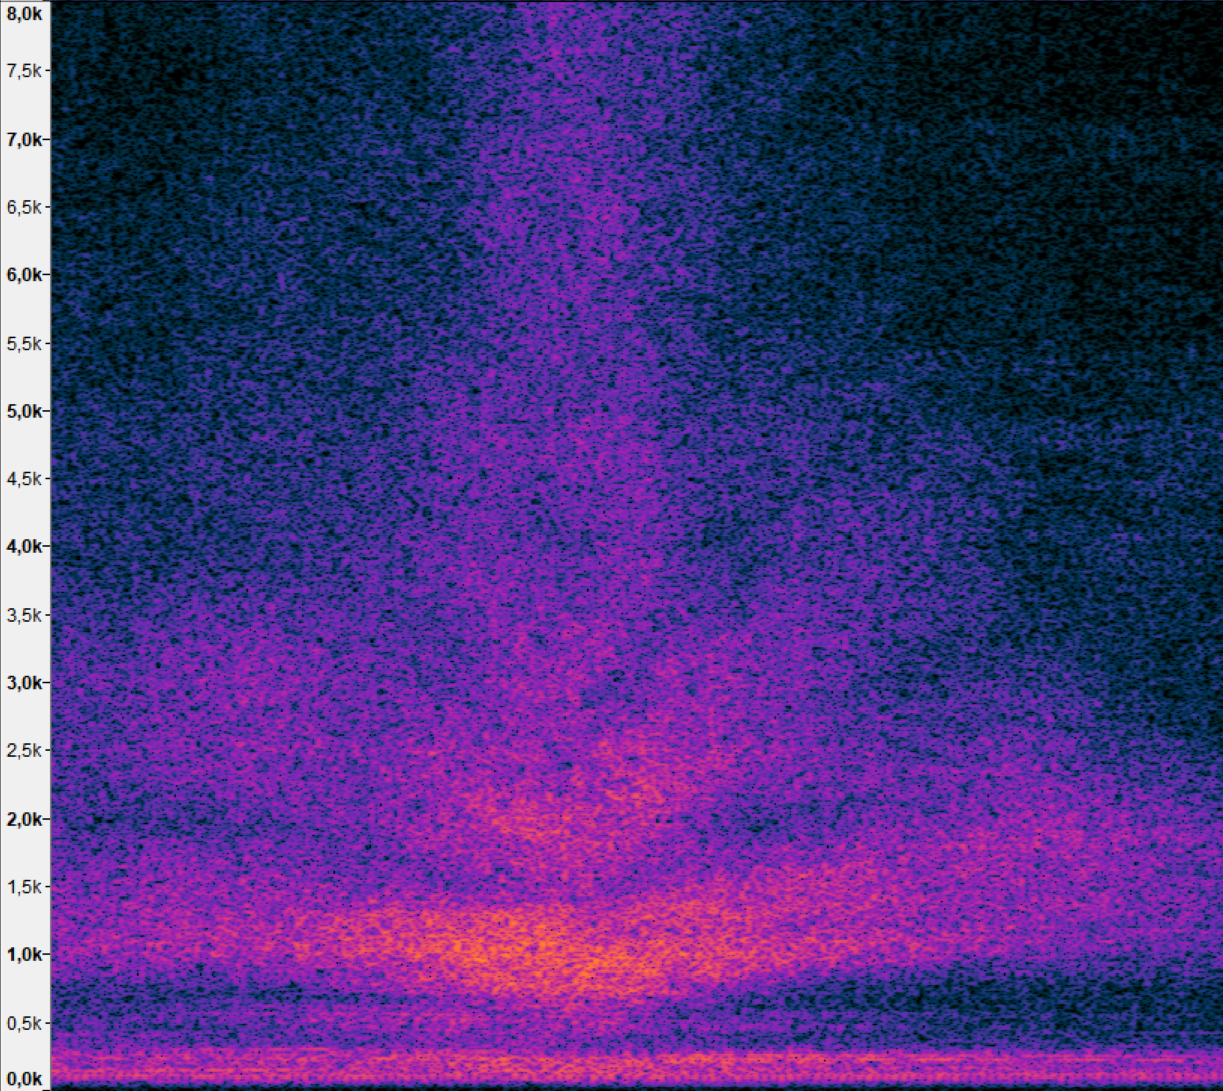
\includegraphics[width=.8\linewidth]{Frequenzen}
        \caption{Spektrogramm}
    \end{subfigure}
    \begin{subfigure}{.5\textwidth}
        \centering
        \includegraphics[width=.8\linewidth]{Tonhöhe(EAC)}
        \caption{Tonhöhe (EAC)}
        \label{img:spectrum_b}
    \end{subfigure}
    \caption{Ergebnisse Spektrumanalysator Reifengeräusche}
    \label{img:spectrumanalyzer}
\end{figure}

\autoref{img:spectrum_b} wurde nachbearbeitet. Die pinkfarbene Linie zeigt den Verlauf der Tonhöhe über Zeit und kann als Frequenzgraph interpretiert werden. Ab der tiefsten Stelle des Graphen ist das vorbeifahrende Kfz am nächsten zum Mikrofon.

Beim Vergleich mit einem theoretisch berechneten Frequenzgraph (\autoref{fig:frequencyplot}) fällt auf, dass die aufgenommene Frequenz der Reifengeräusche vor Vorbeifahren (in der Beispielabbildung bei \(t = 10 s\)) nicht höher ist als nach dem Vorbeifahren, sondern bei niedrigerem Abstand geringer ist. Es konnte keine wissenschaftliche Erarbeitung dieses Phänomens gefunden werden, am wahrscheinlichsten ist jedoch eine Reflexion der akustischen Wellen am Boden, die mit den direkt zum Mikrofon laufenden Wellen interferieren und somit hohe Frequenzen auslöschen. Aufgrund dieser unklaren Messergebnisse kann dieser Ansatz jedoch nicht weiterverfolgt werden.

\subsubsection{Verwendung der Motorgeräusche}

\begin{figure}[h]
    \centering
    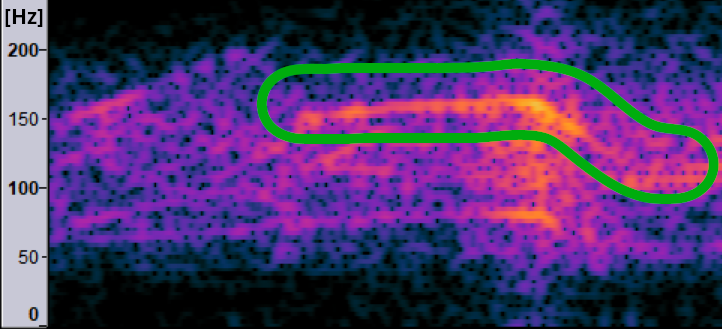
\includegraphics[width=.6\linewidth]{SpektrogrammMotor}
    \caption{Spektrogramm Motorgeräusche}
    \label{fig:spectrum_motor}
\end{figure}

Nachdem sich die Reifengeräusche als unbrauchbar erwiesen haben, ist nun der nächste Ansatz, die Motorgeräusche aufgrund der eindeutigeren Tonhöhe -- anstatt eines Rauschens -- zu analysieren. Hierfür wird ein Tiefpass mit einer Grenze von \(150 Hz\) auf die Audiospur gelegt, um jegliche Reifengeräusche herauszufiltern. Bei der manuellen Analyse stellt sich jedoch heraus, dass selbst die besten Aufnahmen unbrauchbar sind: Der in \autoref{fig:spectrum_motor} grün umrandete Frequenzverlauf stellt die aufgenommenen Motorgeräusche dar, bei denen die Dopplerverschiebung sichtbar ist. Zwar beinhaltet die Aufnahme vor dem Vorbeifahren des Kfz eindeutige Motorgeräusche, allerdings gibt es keine Messpunkte bei Entfernung des Fahrzeugs (hinter dem „Knick“ im Spektrogramm verschwindet die helle, gelbe Linie). Die Motorgeräusche, die direkt mit der Motordrehzahl zusammenhängen, konnten vom verwendeten Handymikrofon gar nicht aufgezeichnet werden, vermutlich unterläge es jedoch den gleichen Einschränkungen wie die aufgezeichneten Oberwellen. Somit kann auch diese Variante der Geschwindigkeitsbestimmung nicht verwendet werden.

\subsection{Analyse der Audiodaten via Lautstärkeänderung}


Das morgen im Freien irgendwie ausprobieren
-> Schallquelle nicht gerichtet (z.B. Lautsprecher zeigt nach oben, also in die Vertikale)
-> Die Abstandsmessung erfolgt in der Horizontalen

\section{Ergebnisse}

\section{Ergebnisdiskussion}

Nachteil: bei dichtem Verkehr eine Trennung der Fahrzeuge ermöglicht wird.

In halliger Umgebung gilt das 1/r-Gesetz nur eingeschränkt: \dots
(siehe Wikipedia-Artikel "Schalldruck\#Abstandsabhängigkeit")

\section{Zusammenfassung}

\newpage

\section{Abbildungsverzeichnis}
\listoffigures

\section{Quellen- und Literaturverzeichnis}

\printbibliography

\section{Unterstützungsleistungen}

\end{document}
